\documentclass[12pt,a4paper]{article}
\usepackage{parskip}
\usepackage{pdfpages}
\usepackage{hyperref}
\usepackage{amsmath}
\usepackage{pgfplots}
\usepackage{caption}
\usepackage{subcaption}
\usepackage[margin=.6in]{geometry}

\usepgfplotslibrary{fillbetween}

\begin{document}
\section*{Question 1}
\label{sec:question_1}

\begin{figure}[h!]
\captionsetup[subfigure]{font=footnotesize}
\centering
\resizebox {3.5in} {!} {
\subcaptionbox*{$\mu_{A_1}$}[.5\textwidth]{%
\begin{tikzpicture}[
  declare function={
    func(\x)= (\x<2) * (0)   +
     and(\x>=2, \x<=5) * ((\x-2)/3)     +
     and(\x>5,  \x<=8) * ((8-x)/3) +
                (\x>8) * (0);
  }
]
\begin{axis}[
  axis x line=middle, axis y line=middle,
  ymin=0, ymax=1.33, ytick={0,0.33,0.66,1},
  xmin=0, xmax=12, xtick={0,...,12}, xlabel=$x$,
]
\pgfplotsinvokeforeach{4}{
  \draw[dashed] ({rel axis cs: 0,0} -| {axis cs: #1, 0}) -- ({rel axis cs: 0,1} -| {axis cs: #1, 0});}
\addplot[blue, domain=0:12]{func(x)};
\node[label={180:{0.66}},circle,fill,inner sep=2pt] at (axis cs:4,0.66) {};
\end{axis}
\end{tikzpicture}}}
\resizebox {3.5in} {!} {
\subcaptionbox*{$\mu_{B_1}$}[.5\textwidth]{%
\begin{tikzpicture}[
  declare function={
    func(\x)= (\x<5) * (0)   +
     and(\x>=5, \x<=8) * ((\x-5)/3)     +
     and(\x>8,  \x<=11) * ((11-x)/3) +
                (\x>11) * (0);
  }
]
\begin{axis}[
  axis x line=middle, axis y line=middle,
  ymin=0, ymax=1.33, ytick={0,0.33,0.66,1},
  xmin=0, xmax=12, xtick={0,...,12}, xlabel=$y$,
]
\pgfplotsinvokeforeach{8}{
  \draw[dashed] ({rel axis cs: 0,0} -| {axis cs: #1, 0}) -- ({rel axis cs: 0,1} -| {axis cs: #1, 0});}
\addplot[blue, domain=0:12]{func(x)};
\node[label={180:{1}},circle,fill,inner sep=2pt] at (axis cs:8,1) {};
\end{axis}
\end{tikzpicture}}}
\end{figure}
The strength of these two rules is 0.66 and the resulting and the cut on $\mu_{C_1}$ will occur at the max, which is 1.

\begin{figure}[h!]
\centering
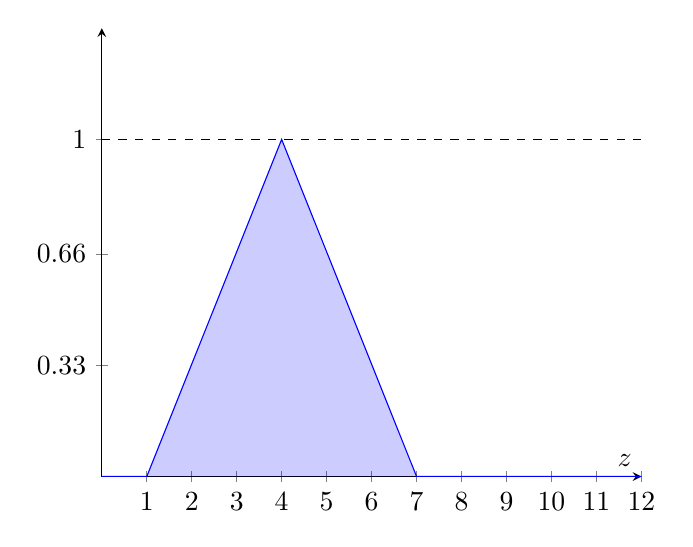
\begin{tikzpicture}[
  declare function={
    func(\x)= (\x<1) * (0)   +
     and(\x>=1, \x<=4) * ((\x-1)/3)     +
     and(\x>4,  \x<=7) * ((7-x)/3) +
                (\x>7) * (0);
  }
]
\begin{axis}[
  axis x line=middle, axis y line=middle,
  ymin=0, ymax=1.33, ytick={0,0.33,0.66,1},
  xmin=0, xmax=12, xtick={0,...,12}, xlabel=$z$,
]
\addplot[blue, domain=0:12, fill=blue, fill opacity=0.2]{func(x)};
  \draw[dashed] ({axis cs: 0, 1}) -- ({axis cs: 12, 1});
\end{axis}
\end{tikzpicture}
\caption*{$\mu_{C_1}$}
\end{figure}

\newpage


\begin{figure}[h!]
\captionsetup[subfigure]{font=footnotesize}
\centering
\resizebox {3.5in} {!} {
\subcaptionbox*{$\mu_{A_2}$}[.5\textwidth]{%
\begin{tikzpicture}[
  declare function={
    func(\x)= (\x<3) * (0)   +
     and(\x>=3, \x<=6) * ((\x-3)/3)     +
     and(\x>6,  \x<=9) * ((9-x)/3) +
                (\x>9) * (0);
  }
]
\begin{axis}[
  axis x line=middle, axis y line=middle,
  ymin=0, ymax=1.33, ytick={0,0.33,0.66,1},
  xmin=0, xmax=12, xtick={0,...,12}, xlabel=$x$,
]
\pgfplotsinvokeforeach{4}{
  \draw[dashed] ({rel axis cs: 0,0} -| {axis cs: #1, 0}) -- ({rel axis cs: 0,1} -| {axis cs: #1, 0});}
\addplot[blue, domain=0:12]{func(x)};
\node[label={180:{0.33}},circle,fill,inner sep=2pt] at (axis cs:4,0.33) {};
\end{axis}
\end{tikzpicture}}}
\resizebox {3.5in} {!} {
\subcaptionbox*{$\mu_{B_2}$}[.5\textwidth]{%
\begin{tikzpicture}[
  declare function={
    func(\x)= (\x<4) * (0)   +
     and(\x>=4, \x<=7) * ((\x-4)/3)     +
     and(\x>7,  \x<=10) * ((10-x)/3) +
                (\x>10) * (0);
  }
]
\begin{axis}[
  axis x line=middle, axis y line=middle,
  ymin=0, ymax=1.33, ytick={0,0.33,0.66,1},
  xmin=0, xmax=12, xtick={0,...,12}, xlabel=$y$,
]
\pgfplotsinvokeforeach{8}{
  \draw[dashed] ({rel axis cs: 0,0} -| {axis cs: #1, 0}) -- ({rel axis cs: 0,1} -| {axis cs: #1, 0});}
\addplot[blue, domain=0:12]{func(x)};
\node[label={360:{0.66}},circle,fill,inner sep=2pt] at (axis cs:8,0.66) {};
\end{axis}
\end{tikzpicture}}}
\end{figure}
The strength of these two rules is 0.33 and the resulting and the cut on $\mu_{C_1}$ will occur at the max, which is 0.66.

\begin{figure}[h!]
\centering
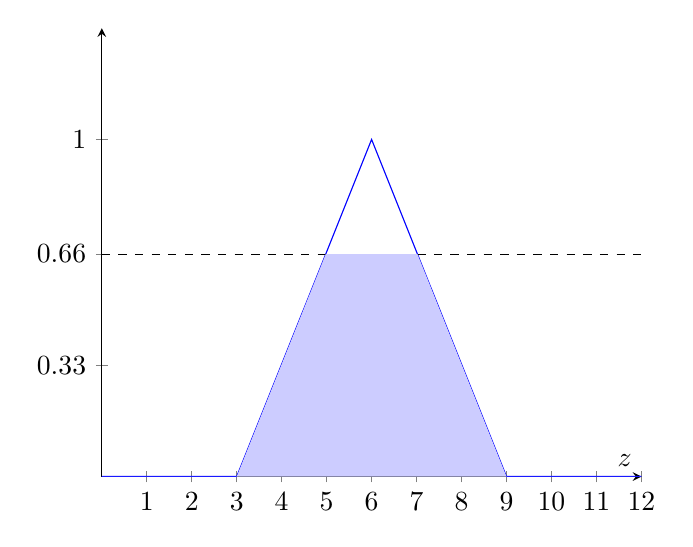
\begin{tikzpicture}[
  declare function={
    func(\x)= (\x<3) * (0)   +
     and(\x>=3, \x<=6) * ((\x-3)/3)     +
     and(\x>6,  \x<=9) * ((9-x)/3) +
                (\x>9) * (0);
  }
]
\begin{axis}[
  axis x line=middle, axis y line=middle,
  ymin=0, ymax=1.33, ytick={0,0.33,0.66,1},
  xmin=0, xmax=12, xtick={0,...,12}, xlabel=$z$,
]
\addplot[name path=f, blue, domain=0:12]{func(x)};
\addplot[name path=cut, black, dashed, domain=0:12]{0.66};

\path[name path=axis] ({axis cs: 0, 0}) -- ({axis cs: 12, 0});

\fill[blue!20!white,intersection segments={of=f and cut,sequence={A0 -- B1 -- A2}}]
    -- (axis cs:12,\pgfkeysvalueof{/pgfplots/ymin})
    -- (axis cs:0,\pgfkeysvalueof{/pgfplots/ymin})
    -- cycle
;
\end{axis}
\end{tikzpicture}
\caption*{$\mu_{C_2}$}
\end{figure}

\begin{figure}[h!]
\centering
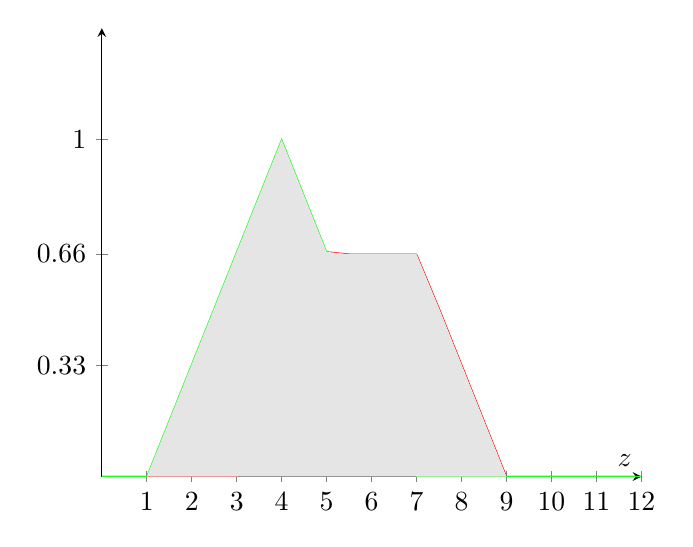
\begin{tikzpicture}[
  declare function={
    func1(\x)= (\x<3) * (0)   +
     and(\x>=3, \x<=5) * ((\x-3)/3)     +
     and(\x>5,  \x<=7) * (0.66) +
     and(\x>7,  \x<=9) * ((9-x)/3) +
                (\x>9) * (0);
  },
  declare function={
    func2(\x)= (\x<1) * (0)   +
     and(\x>=1, \x<=4) * ((\x-1)/3)     +
     and(\x>4,  \x<=7) * ((7-x)/3) +
                (\x>7) * (0);
  }
]
\begin{axis}[
  axis x line=middle, axis y line=middle,
  ymin=0, ymax=1.33, ytick={0,0.33,0.66,1},
  xmin=0, xmax=12, xtick={0,...,12}, xlabel=$z$,
]
\addplot[name path=f1, red, domain=0:12]{func1(x)};
\addplot[name path=f2, green, domain=0:12]{func2(x)};

\path[name path=axis] ({axis cs: 0, 0}) -- ({axis cs: 12, 0});

\fill[black!10!white,intersection segments={of=f1 and f2,sequence={A0 -- B1 -- A2}}]
    -- (axis cs:12,\pgfkeysvalueof{/pgfplots/ymin})
    -- (axis cs:0,\pgfkeysvalueof{/pgfplots/ymin})
    -- cycle
;
\end{axis}
\end{tikzpicture}
\caption*{output}
\end{figure}

In this instance we have only one maximum at 4 so the mean of maxima is 4, giving us the defuzzified output at $t_1$.

When calculating for the centroid of area a slightly different answer occurs.

\begin{align*}
	c &= \frac{\int c\mu_c(c)\delta c}{\int \mu_c(c)\delta c}\\
		&= \frac{\int_1^5 \frac{x-1}{3}x\delta x + \int_5^70.66x\delta x + \int_7^9 \frac{9-x}{3}x\delta x}
			{\int_1^5 \frac{x-1}{3}\delta x + \int_5^70.66\delta x + \int_7^9 \frac{9-x}{3}\delta x}\\
		&= \frac{22.8089}{4.6533}\\
		&= 4.9016
\end{align*}

The centroid of area is slightly higher because the mean of maxima disregards the values outside of its single peak. This is also why the centroid of area returns a more accurate result.

\section*{Question 2}
\label{sec:question_2}
\subsection*{a)}
\label{sub:a_}
\subsubsection*{i)}
\label{ssub:i_}
Classical:

\begin{tabular}{c | c c c c c c c}
f\textbackslash K & $1e+3$ & $1e+4$ & $1e+5$ & $5e+5$ & $1e+6$ & $5e+6$ & $1e+7$\\
\hline
100  & 1  & 0.8  & 0.5  & 0.2  & 0  & 0.2  & 0.8 \\
200  & 1  & 0.8  & 0.5  & 0.2  & 0  & 0.2  & 0.8 \\
500  & 1  & 0.8  & 0.5  & 0.2  & 0.2  & 0.2  & 0.8 \\
800  & 1  & 0.8  & 0.5  & 0.5  & 0.5  & 0.5  & 0.8 \\
1000 & 1  & 0.8  & 0.5  & 0.8  & 1  & 0.8  & 0.8 \\
2000 & 1  & 0.8  & 0.5  & 0.8  & 0.8  & 0.8  & 0.8 \\
5000 & 1  & 0.8  & 0.5  & 0.2  & 0.2  & 0.2  & 0.8 \\
\end{tabular}

\subsubsection*{ii)}
\label{ssub:ii_}
Mamdani:

\begin{tabular}{c | c c c c c c c}
f\textbackslash K & $1e+3$ & $1e+4$ & $1e+5$ & $5e+5$ & $1e+6$ & $5e+6$ & $1e+7$\\
\hline
100  & 0  & 0  & 0  & 0  & 0  & 0  & 0 \\
200  & 0  & 0  & 0  & 0  & 0  & 0  & 0 \\
500  & 0  & 0.2  & 0.2  & 0.2  & 0.2  & 0.2  & 0.2 \\
800  & 0  & 0.2  & 0.5  & 0.5  & 0.5  & 0.5  & 0.2 \\
1000 & 0  & 0.2  & 0.5  & 0.8  & 1  & 0.8  & 0.2 \\
2000 & 0  & 0.2  & 0.5  & 0.8  & 0.8  & 0.8  & 0.2 \\
5000 & 0  & 0.2  & 0.2  & 0.2  & 0.2  & 0.2  & 0.2 \\
\end{tabular}

\subsubsection*{iii)}
\label{ssub:iii_}
Product:

\begin{tabular}{c | c c c c c c c}
f\textbackslash K & $1e+3$ & $1e+4$ & $1e+5$ & $5e+5$ & $1e+6$ & $5e+6$ & $1e+7$\\
\hline
100   & 0  & 0.0  & 0.0  & 0.0  & 0  & 0.0  & 0.0 \\
200   & 0  & 0.0  & 0.0  & 0.0  & 0  & 0.0  & 0.0 \\
500 & 0.0  & 0.04  & 0.1  & 0.16  & 0.2  & 0.16  & 0.04 \\
800 & 0.0  & 0.1  & 0.25  & 0.4  & 0.5  & 0.4  & 0.1 \\
1000   & 0  & 0.2  & 0.5  & 0.8  & 1  & 0.8  & 0.2 \\
2000 & 0.0  & 0.16  & 0.4  & 0.64  & 0.8  & 0.64  & 0.16 \\
5000 & 0.0  & 0.04  & 0.1  & 0.16  & 0.2  & 0.16  & 0.04 \\
\end{tabular}

\subsection*{b)}
\label{sub:b_}
\begin{align*}
	R &=\begin{bmatrix}
		1  & 0.8  & 0.5  & 0.2  & 0  & 0.2  & 0.8 \\
		1  & 0.8  & 0.5  & 0.2  & 0  & 0.2  & 0.8 \\
		1  & 0.8  & 0.5  & 0.2  & 0.2  & 0.2  & 0.8 \\
		1  & 0.8  & 0.5  & 0.5  & 0.5  & 0.5  & 0.8 \\
		1  & 0.8  & 0.5  & 0.8  & 1  & 0.8  & 0.8 \\
		1  & 0.8  & 0.5  & 0.8  & 0.8  & 0.8  & 0.8 \\
		1  & 0.8  & 0.5  & 0.2  & 0.2  & 0.2  & 0.8 \\
	\end{bmatrix}\\
	K' &=\begin{bmatrix}
		0\\
		0.8\\
		0.2\\
	\end{bmatrix}\\
	f_1 &= R \circ K'\\
		&= \max_{rows} \left(\min_{cols} \left(K', R\right)\right)\\
		&= \max_{cols} \left(\min_{cols} \left(
		\begin{bmatrix}
			0\\
			0.8\\
			0.2\\
		\end{bmatrix},
	\begin{bmatrix}
		1  & 0.8  & 0.5  & 0.2  & 0  & 0.2  & 0.8 \\
		1  & 0.8  & 0.5  & 0.2  & 0  & 0.2  & 0.8 \\
		1  & 0.8  & 0.5  & 0.2  & 0.2  & 0.2  & 0.8 \\
		1  & 0.8  & 0.5  & 0.5  & 0.5  & 0.5  & 0.8 \\
		1  & 0.8  & 0.5  & 0.8  & 1  & 0.8  & 0.8 \\
		1  & 0.8  & 0.5  & 0.8  & 0.8  & 0.8  & 0.8 \\
		1  & 0.8  & 0.5  & 0.2  & 0.2  & 0.2  & 0.8 \\
	\end{bmatrix}
		\right)
		\right)\\
	&= \max_{cols} \left(
	\begin{bmatrix}
		0 & 0 & 0 & 0 & 0 & 0 & 0\\
		0.8 & 0.8 & 0.5 & 0.2 & 0 & 0.2 & 0.8\\
		0.2 & 0.2 & 0.2 & 0.2 & 0.2 & 0.2 & 0.2\\
	\end{bmatrix}
		\right)\\
	&= \begin{bmatrix}
		0.8 & 0.8 & 0.5 & 0.2 & 0.2 & 0.2 & 0.8\\
		\end{bmatrix}\\
\end{align*}

\section*{Question 3}
\label{sec:question_3}
\begin{align*}
	T_{300} &= \left\{\frac{0}{LW} + \frac{1}{HG}\right\} \\
	M_{800} &= \left\{\frac{0}{SM} + \frac{1}{LG}\right\} \\
	P_{1.3} &= \left\{\frac{0.2}{FR} + \frac{0.8}{NR}\right\} \\
\end{align*}
Finding the pertinent rules:
\begin{align*}
	HG\times LG \times NR = \frac{0.8}{RD}\\
	HG\times LG \times FR = \frac{0.2}{RD}\\
\end{align*}

NOTE: need to figure out which rule to apply for now assume that both reference the RD value and hope that order is conserved.




































\end{document}
